
\documentclass[a4paper, 11pt]{article}

% Fonts 
\usepackage{opensans}
\usepackage{amsfonts}
\usepackage{montserrat}
\usepackage{amsmath}

\setmainfont{opensans}
\usepackage[mathrm=sym]{unicode-math}
% \setmathfont[Path=font/,mathrm=sym]{FiraMath-Regular}
\setmathfont[Path=font/,mathrm=sym]{LatoMath}

\newfontfamily{\montserrateb}{Montserrat SemiBold}
\newfontfamily{\montserratb}{Montserrat Bold}
\newfontfamily{\montserrat}{Montserrat Regular}
\newfontfamily{\montserratl}{Montserrat Light}
% \DeclareMathAlphabet{\mathcal}{OMS}{cmbrs}{m}{n}

% \usepackage[mathrm=sym]{unicode-math}
% \setmainfont{opensans}
% \setmathfont{Fira Math}

% \newfontfamily{\montserrateb}{Montserrat SemiBold}
% \newfontfamily{\montserratb}{Montserrat Bold}
% \newfontfamily{\montserrat}{Montserrat Regular}
% \newfontfamily{\montserratl}{Montserrat Light}
% \DeclareMathAlphabet{\mathcal}{OMS}{cmbrs}{m}{n}
% \setmathfont{Latin Modern Math}[range={\vdots}]

% \autoref
\usepackage{hyperref}

% Use for [H] option for figures to force in text placement
\usepackage{float}

% Captioning figures
\usepackage{caption}

% Subfigures
\usepackage{subcaption}

% For extending contents beyond margins
\usepackage{scrextend}

% For tables \midrule ect
\usepackage{booktabs}

% Colours
\usepackage[table,xcdraw]{xcolor}
\definecolor{accentcolor}{HTML}{a13640}

% Change label in enumerate 
\usepackage{enumitem}

% Section settings
\usepackage{titlesec}
\titleformat{\section}
{\LARGE\montserrateb}
{\thesection.}{0.5em}{}

\titleformat{\subsection}
{\large\montserratb}
{\thesubsection.}{0.5em}{}

% Adjust document dimensions
\ExecuteOptions{a4paper}
\addtolength{\oddsidemargin}{-3cm}
\addtolength{\evensidemargin}{-3cm}
\addtolength{\topmargin}{-3cm}
\addtolength{\textwidth}{6cm}
\addtolength{\textheight}{4.5cm}
\addtolength{\textheight}{1.5cm}
\addtolength{\headsep}{-0.5cm}
% \addtolength{\footskip}{-1cm}
\parindent0pt
\parskip=4pt



\usepackage{matlab-prettifier}
\usepackage{graphicx}
\usepackage{mdframed}

% Creates coloured title box
\newcommand{\thetop}[5]{
	\begin{addmargin}[\oddsidemargin]{\oddsidemargin}
		\colorbox{#5}{\color{white}
			\hbox to \paperwidth{
				\vbox {
					\begin{center}
						{\large\montserratl #1}\\
						\vspace{4pt}
						{\huge\montserratb #2}\\
						{\montserratb #3}\\
						\vspace{-0.5em}
						\rule{20em}{1pt}

						{\large\montserratl
							#4
						}
					\end{center}
				}
			}
		}
	\end{addmargin}
}

\newcommand{\NN}{\mathbb{N}}
\newcommand{\ZZ}{\mathbb{Z}}
\newcommand{\RR}{\mathbb{R}}
\newcommand{\CC}{\mathbb{C}}
\newcommand{\dydt}{\frac{dy}{dt}}
\newcommand{\dxdt}{\frac{dx}{dt}}
\def\set#1{\left\{ #1 \right\}}
\def\eval#1#2{\left\ #1\right|_{#2}}

\def\pp#1#2{\frac{\partial #1}{\partial #2}}
\def\dd#1#2{\frac{\,d#1}{\,d#2}}
\def\abs#1{\left|#1\right|}
\def\conj#1{\overline{#1}}

\usepackage{multicol}
\usepackage{tikz}
\usepackage{pgfplots}
\usetikzlibrary {graphs,graphdrawing} \usegdlibrary {force} 
\usetikzlibrary{graphs.standard}
\usetikzlibrary{positioning, 
                quotes}
\usegdlibrary {circular}

\usepackage{pst-platon}

\usepackage{comment}

\begin{comment}
	Q1:  sol
	Q2:  sol 
	Q3a: sol
	Q3b:  
	Q4:  sol
	Q5a: sol
	Q5b: sol
	Q6:  sol
	Q7:  sol
\end{comment}

\begin{document}
\thetop{Robert Christie}{MATHS 326}{S1 2024}{Assignment 2\\Due: 19-04-2024}{accentcolor}

\begin{multicols*}{2}
	\section*{Q1}
	Consider the following weighted graph:
	\begin{center}
		\begin{tikzpicture}[
				node distance = 15mm and 15mm,
				% V/.style = {circle, draw, fill=gray!30},
				V/.style = {circle, draw},
				every edge quotes/.style = {auto, font=\footnotesize, sloped}
			]
			\begin{scope}[nodes=V]
				\node (A)   {A};
				\node (B) [above right=of A]    {B};
				\node (C) [below right=of B]    {C};
			\end{scope}

			\draw
			(A)  edge["$2$"] (B)
			(B)  edge["$-2$"] (C);

			\draw
			(A)  edge["$1$"] (C);
		\end{tikzpicture}
	\end{center}
	Applying Dijkstra's Algorithm starting from $v=A$:
	\begin{itemize}
		\item
		      Initial stage: We set:
		      \[
			      R=\emptyset,\quad
			      \delta(v)=\begin{cases}
				      0      & v=A \\
				      \infty & v=B \\
				      \infty & v=C
			      \end{cases}
		      \]
		      Also set $A$ to be the current vertex.

		\item Iteration 1: Add $A$ to $R$, and update $\delta$ giving:
		      \[
			      R=\set{A},\quad
			      \delta(v)=\begin{cases}
				      0 & v=A \\
				      2 & v=B \\
				      1 & v=C
			      \end{cases}
		      \]
		      Then we set $C$ as the current vertex as it has the smallest $\delta$ of the unvisited vertices.

		\item Iteration 2: We add $C$ to $R$, and update $\delta$ giving:
		      \[
			      R=\set{A,C},\quad
			      \delta(v)=\begin{cases}
				      \hphantom{-}0 & v=A \\
				      -1            & v=B \\
				      \hphantom{-}1 & v=C
			      \end{cases}
		      \]
		      Now that $C$ has been visited, the algorithm will not alter $\delta(C)$ any further.
	\end{itemize}
	Thus, the final value of $\delta(C)=1$. However, the actual shortest path from $A$ to $C$ is $A$---$B$---$C$ with length $0$. So Dijkstra's algorithm doesn't always find shortest paths if positive and negative edge weights are allowed.

	\section*{Q2}

	Let $G=(V,E,w)$ be a weighted graph with weight function $w$.

	Proof by contradiction:

	Assume that $G$ does not have a unique MST, thus we can find two distinct spanning trees $T$ and $T'$ with the same minimal weight. Since $T$ and $T'$ are distinct, there must exist an edge in one (but not both) of $T$ and $T'$, let $e$ be such an edge with minimal $w(e)$ and WLOG assume $e$ is in $T$ but not in $T'$.

	Let $e=\set{u,v}$, since $T'$ is also spanning, there is some other path from $u$ to $v$ in $T'$, so adding $e$ to $T'$ would create a cycle. Because $T$ is a tree, it cannot contain the cycle, so some other edge $e'$ of the cycle is not in $T$.

	Since $e'$ is also in one but not both of $T$ and $T'$ and $e$ was the smallest edge with this property, we must have $w(e')>w(e)$. However, if we remove $e'$ from $T'$ and insert $e$, we have constructed a new MST with smaller weight, meaning $T$ and $T'$ were not minimal. This is a contradiction so $G$ must have a unique MST.

	\section*{Q3}
	\begin{enumerate}[label=(\alph*)]
		\item Counter example: Consider the following graph:
		      \begin{center}
			      \begin{tikzpicture}[
					      node distance = 15mm and 15mm,
					      % V/.style = {circle, draw, fill=gray!30},
					      V/.style = {circle, draw},
					      every edge quotes/.style = {auto, font=\footnotesize, sloped}
				      ]
				      \begin{scope}[nodes=V]
					      \node (A)   {A};
					      \node (B) [above right=of A]    {B};
					      \node (C) [right=of B]          {C};
					      \node (D) [below right=of C]    {D};
				      \end{scope}

				      \draw[red!70!black]
				      (A)  edge["$\frac12$"] (B)
				      (B)  edge["$\frac12$"] (C)
				      (C)  edge["$\frac12$"] (D);

				      \draw[blue!70!black]
				      (A)  edge["$1$"] (D);

			      \end{tikzpicture}
		      \end{center}
		      In the original weighting, the shortest path from $A$ to $D$ is given by the blue path with weight $1$. Replacing each edge weight with the square would make the red path shortest with weight $\frac 34$, the blue path still has length $1$.

		      \pagebreak
		\item

		      Let $G=(V,E,w)$ be a weighed graph with weight function $W:E\to\RR^+$.

		      Consider any $T_0$ of $G$ and apply Kruskal's algorithm, if edges have the same weight, choose edges in $T_0$ first before looking at other edges. This still follows the definition of Kurskal's algorithm as the order of edges with the same weight is undecided.

		      We claim that this modification of Kruskal's algorithm will output a $T$ with $T=T_0$ when $T_0$ is an MST.

		      Proof by contradiction:

		      \begin{mdframed}
			      Assume that $T_0$ was not output, therefore at some point an edge $e$ was added to $T_0$ where $e$ not in $T_0$. Consider the first such edge added.

			      Until $e$ was added, $T$ is a subgraph of $T_0$, and all edges in $T_0$ of weight at most $w(e)$ are already in $T$. Since Kruskal's algorithm added $e$, this did not create a cycle in $T$.

			      Now consider adding $e=\set{u,v}$ to $T_0$, this must create a cycle since $T_0$ is connected, so there is already a path from $u$ to $v$.

			      When $e$ was added, $T$ already contained all the edges of $C$ with weight at most $w(e)$ and did not contain a cycle. Hence, we can break the cycle by removing an edge $e'$ from $C$ with $w(e')>w(e)$.

			      This creates a spanning tree with smaller weight than $T_0$, we have a contradiction as $T_0$ was already an MST.

			      Therefore, Kruskal's algorithm will output $T$ with $T=T_0$ when $T_0$ is a MST.
		      \end{mdframed}

		      Now consider some strictly increasing function $f:\RR^+\to\RR^+$. Consider any MST $T_0$ in $G$ and $G'=(V,E,f\circ w)$.

		      Consider Kurskal's algorithm applied to $G$ and $G'$ choosing edges in $T_0$ first when edges have the same weight.
		      \begin{mdframed}
			      Step 1: Both initialise $T$ to the same spanning subgraph with no edges.

			      Step 2: Both algorithms will consider the edges in the same order as $f$ is increasing, so it preserves the order of $w$.

			      Step 3: We can apply induction (base case step 1) to see that the same edges will be added as at each iteration: If the same edges were added to $T$ previously, then $e$ creates a cycle in $T$ as a subgraph of $G'$ if and only if it created a cycle in $G$ as cycles aren't affected by the weighting function.

			      Therefore, Kurskal's algorithm on $G'$ will output the same $T=T_0$ as it does on $G$.
		      \end{mdframed}

		      Since $x^2$ and $\sqrt{x}$ are strictly increasing functions  $\RR^+\to\RR^+$, applying our previous working:

		      \begin{itemize}
			      \item
			            Any MST in $G$ with weighting function $w$ is also a weighting function in $G'$ with weighting function $w'=w^2$.

			      \item
			            We also see that any MST in $G'$, is a MST in $G$ with weighting function $w=\sqrt{w'}$.
		      \end{itemize}

		      Thus, we have shown equivalence.


		      %   Claim: If $G=(V,E,w)$ with $|E|=m$, then WLOG let:
		      %   $$w:E \to \set{1,\dots, m }$$
		      %   Preserving equality and inequality between edge weights. Now for some MST $T$ define $E_T$ be the edges in $T$ define:
		      %   $$W_T(i)=\set{e\in E(T): w(e)=i}$$
		      %   We claim that for any fixed $G$ and $1\leq i \leq m$, $|E_i|$ is constant with respect to the choice of $T$.

		      %   Proof: Apply strong induction on $i$ show that for any $j\leq i$, that $W_T(j)$ is constant with respect to the MST $T$ for any fixed graph $G=(V,E)$ of $|V|=n$.

		      %   \textbf{Base Case:} $i<1$ Vacuously true.

		      %   \textbf{Inductive Step:} Let $W^*$ be defined as:
		      %   $$W^*= \bigcup_{j=1}^{i-1} W_T(j)$$
		      %   Consider the forest induced on $T$ by $W^*$, apply the inductive hypothesis to each tree (connected component) in the forest, all trees have





		      %   %   Proof: Let $G=(V,E,w)$ be a weight graph with original weighting function $w:E\to \RR^+$. Since a minimum spanning tree $M$ of $G$ is a forest with $p=\abs V$ vertices and $q=\abs E$ edges and $c=1$ connect components, By \textit{lemma 0.1}, $p-q=c$ so $q=p-c=p-1$.


		      %   %   1=>2:
		      %   %   Let $M$ be a MST in $w$. If $M$ is not an MST in


		      %   %   2=>1:

		      %   %   %   Assume that $M$ is not a MST in the new weighting function. Then some other $M'$ is a MST in the new weighting, but not in the old weighting.
		      %   %   %   \[
		      %   %   %       \sum_{e\in M}w(e) < \sum_{e\in M'}w(e)
		      %   %   %   \]


		      %   %   1, 1, 8 
		      %   %   2, 2, 2 

		      %   \textcolor{red}{Proof maximum cycle property.}

		      %   Claim: If $G=(V,E,w)$ with $|E|=m$, then for any MST $T$, then WLOG let:
		      %   $$w:E \to \set{1,\dots, m }$$
		      %   Preserving equality and inequality between edge weights. Now for $E_T$ be the edges in $T$ define:
		      %   $$E_i=\set{e\in E(T): w(e)=i}$$
		      %   We claim that for $1\leq i \leq m$, for any MST $T$, $|E_i|$ is constant.

		      %   Direct proof:

		      %   Consider any two MST's, $T$ and $T'$ and define $E_i'$ as:
		      %   $$E_i'=\set{e\in E_{T'}: w(e)=i }$$
		      %   We show that $|E_i'|=|E_i|$ via induction:

		      %   \textbf{Base Case:} $i<1$ vacuously true.

		      %   \textbf{Induction Step:} Assume that:
		      %   $$|E_j'|=|E_j|$$
		      %   For any $j<i$, we show via contraction that $|E_i'|=|E_i|$. Assume WLOG $\abs{E_i'}>\abs{E_i}$ therefore:
		      %   $$E_i^*=E_i'\setminus E_i\neq \emptyset$$
		      %   Then for each $e\in E^*$ consider the subgraph $T+e$.

		      %   Let $e=\set{u,v}$, since $e\notin E_i$, there is already a path from $u$ to $v$ in $T$, and so we have created a cycle $C$.

		      %   If $C$ contains an edge $f$ with $w(f)>w(e)$, then $T-f+e$ is a spanning tree with smaller weight which is a contradiction.

		      %   Otherwise, we have $w(f)\leq w(e)$.


		      %   \textcolor{red}{BIG GAP, SHOW OTHER $f\in C$ WITH $w(f)=w(e)$ }

		      %   Now consider adding each edge $e\in C$ where $w(e)<i$ to $T'$,










		      %   %   Claim: If $G=(V,E,w)$ with some $w:E\to\RR^+$, then $T$ is a minimum spanning tree on $G$ if and only if it is a minimum spanning tree in $G'=(V,E,f\circ w)$ where $f:\RR^+\to\RR^+$ is strictly increasing.

		      %   %   Proof: Assume that the claim is false.

		      %   %   \textcolor{red}{ASSUME THAT THE WEIGHTS OF $G$ ARE UNIQUE}

		      %   %   Let



	\end{enumerate}

	\section*{Q4}
	First we show ``$1\implies 2$'':
	\begin{mdframed}
		Assume a tree $T=(V,E)$ has a perfect matching. For any $v\in V$, there is some $u\in V$ matched to $v$. This splits $T$ into $n\geq 1$ connected components.

		One of these components $C_1$ must contain $u$, there must be no other edge from $C_1$ to $v$ in $T$ otherwise $T$ would contain a cycle.

		Since $u$ was matched to $v\notin C_1$, any edge from $C_1$ to $u$ was unmatched so restricting $M$ onto $C_1-u$ does not break any matching giving $C_1-u$ a perfect matching.

		Therefore, $C_1$ has an odd number of vertices.

		Each remaining connected $C_i$ did contain a vertex matched to $v$. Since no matched pair has a single vertex in $C_i$, restricting $M$ to $C_i$ gives a perfect matching so $C_i$ has an even number of vertices.

		Thus, $o(T-v)=1$.
	\end{mdframed}

	Now to show the other direction ``$2\implies 1$'', we assume $o(T-v)=1$.  Observe and define the following:
	\begin{itemize}
		\item
		      $T-v$ must contain exactly one odd connected component, call this component $\Theta(v)$.

		\item
		      As $T$ was connected, each connected component $C_i$ contains a $u_i\in V$ adjacent to $v$ in $T$.

		\item
		      There is exactly one such $u_i$ in each component. If this wasn't the case then this would create a cycle in $T$ as $u_i$ and $u_i'$ are already connected in $C_i$, this isn't possible as $T$ is a tree.

		\item
		      Construct the set $M$ containing $e=\set{v,u}$ for each $v\in V$, where $u\in\Theta(v)$ is adjacent to $v$ in $T$.
	\end{itemize}

	We claim that the edges in $M$ are mutually disjoint. Proof by contradiction:



	\begin{mdframed}
		\begin{center}
			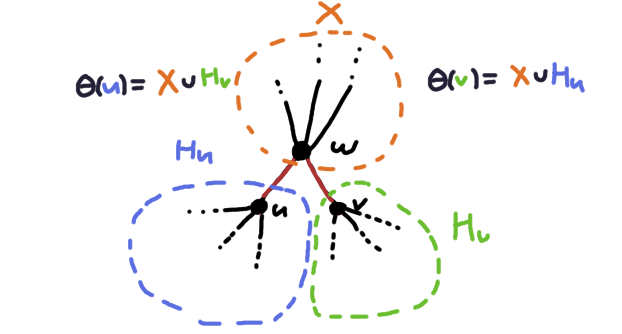
\includegraphics[width=0.75\linewidth]{fig.png}
		\end{center}

		Assume that two edges in $M$ are not disjoint, so some $u,v\in V$ were both paired to some $w$.

		Let $H_u$ be the subgraph of $T$ induced by all the vertices of the even connected components of $T-u$ and the vertex $u$. Notice that $H_u$ is connected as $u$ connected to each of the connected components. Note that $H_u$ has an odd number of vertices as it contains both the even connected components and a singular $u$ (all of which are disjoint). Define $H_v$ in the same way.

		For any $x\in\set{u,v}$ then only $x$ could be connected to a vertex outside of $H_x$, otherwise. If this were not the case and $H_x$ had an edge to some other vertex $y$, then this edge would form a cycle from the existing path through $x$ to $y$, however $T$ cannot contain cycles.

		The subgraphs $H_u,H_v$ are disjoint since $\Theta(u)$ contains $w$ which is still connected to $v$ in $H_v$, thus $H_v$ is a subgraph of $\Theta(u)$ which is not contained in $H_u$.

		Notice that both $H_u$ and $H_v$ contain an odd number of vertices as they contain the even connected components in $T-u$ or $T-v$ as well as $u$ or $v$ respectfully.

		Now consider $T-w$, both $H_u$ and $H_v$ are connected components in $T-w$ as they are not contained in any larger connected component and the only edge in $T$ leaving either subgraph contained $w$.

		Both $H_u$ and $H_v$ have an odd numbers of vertices so $o(T-w)\geq 2$ which is a contradiction.
	\end{mdframed}

	Therefore, $M$ is a matching by definition, however $M$ is also a perfect matching as it clearly contains every $v\in V$.





	\section*{Q5}

	\begin{enumerate}[label=(\alph*)]
		\item
		      Since $G=(V,E)$ is regular, $G$ is $d$-regular for $d=\Delta(G)$. Since $G$ is class 1, there is a $d$-edge colouring $\lambda: E\to C$ with $|C|=d$. For any edge $e_0$ of $G$, consider the matching give by:
		      $$M= \set{e\in E : \lambda(e)=\lambda(e_0)}$$
		      By definition of edge-colouring, the edges of $M$ are mutually disjoint and therefore a valid matching. Since each degree has degree $d$, there are $d$ edges with each of the colours including $\lambda(e_0)$. Thus, every vertex must be contained in $M$ making $M$ a perfect matching. Thus, any $e_0$ is matchable.

		\item
		      The Petersen graph is $3$-regular and was shown to have chromatic index $4$ in \textit{Assignment 1}, thus it is regular and class 2. Consider the following matchings on the Petersen graph where the red edges are the matched edges:
		      \begin{center}
			      \begin{tabular}{cc}
				      \begin{tikzpicture}[every node/.style={draw,circle}]
					      \begin{scope}[shift={(0,-0.75cm)}]
						      \graph[empty nodes, simple necklace layout, clockwise, radius=0.75cm] {
						      A, B, C, D, E;
						      A --[black] C --[red] E --[black] B --[red] D --[black] A;
						      };
					      \end{scope}
					      \graph[empty nodes, simple necklace layout, clockwise, radius=1.5cm] {
					      1--[black]2--[red]3--[black]4--[red]5--[black]1;
					      };
					      \draw[red] (1) -- (A);
					      \draw[black]  (2) -- (B);
					      \draw[black]  (3) -- (C);
					      \draw[black]  (4) -- (D);
					      \draw[black]  (5) -- (E);
				      \end{tikzpicture}
				       &
				      \begin{tikzpicture}[every node/.style={draw,circle}]
					      \begin{scope}[rotate=72]
						      \begin{scope}[shift={(0,-0.75cm)}]
							      \graph[empty nodes, simple necklace layout, clockwise, radius=0.75cm] {
							      A, B, C, D, E;
							      A --[black] C --[red] E --[black] B --[red] D --[black] A;
							      };
						      \end{scope}
						      \graph[empty nodes, simple necklace layout, clockwise, radius=1.5cm] {
						      1--[black]2--[red]3--[black]4--[red]5--[black]1;
						      };
						      \draw[red] (1) -- (A);
						      \draw[black]  (2) -- (B);
						      \draw[black]  (3) -- (C);
						      \draw[black]  (4) -- (D);
						      \draw[black]  (5) -- (E);
					      \end{scope}
				      \end{tikzpicture}
				      \\
				      \begin{tikzpicture}[every node/.style={draw,circle}]
					      \begin{scope}[rotate=144]
						      \begin{scope}[shift={(0,-0.75cm)}]
							      \graph[empty nodes, simple necklace layout, clockwise, radius=0.75cm] {
							      A, B, C, D, E;
							      A --[black] C --[red] E --[black] B --[red] D --[black] A;
							      };
						      \end{scope}
						      \graph[empty nodes, simple necklace layout, clockwise, radius=1.5cm] {
						      1--[black]2--[red]3--[black]4--[red]5--[black]1;
						      };
						      \draw[red] (1) -- (A);
						      \draw[black]  (2) -- (B);
						      \draw[black]  (3) -- (C);
						      \draw[black]  (4) -- (D);
						      \draw[black]  (5) -- (E);
					      \end{scope}
				      \end{tikzpicture}
				       &
				      \begin{tikzpicture}[every node/.style={draw,circle}]
					      \begin{scope}[rotate=216]
						      \begin{scope}[shift={(0,-0.75cm)}]
							      \graph[empty nodes, simple necklace layout, clockwise, radius=0.75cm] {
							      A, B, C, D, E;
							      A --[black] C --[red] E --[black] B --[red] D --[black] A;
							      };
						      \end{scope}
						      \graph[empty nodes, simple necklace layout, clockwise, radius=1.5cm] {
						      1--[black]2--[red]3--[black]4--[red]5--[black]1;
						      };
						      \draw[red] (1) -- (A);
						      \draw[black]  (2) -- (B);
						      \draw[black]  (3) -- (C);
						      \draw[black]  (4) -- (D);
						      \draw[black]  (5) -- (E);
					      \end{scope}
				      \end{tikzpicture}
				      \\
				      \multicolumn{2}{c}{
					      \begin{tikzpicture}[every node/.style={draw,circle}]
						      \begin{scope}[rotate=288]
							      \begin{scope}[shift={(0,-0.75cm)}]
								      \graph[empty nodes, simple necklace layout, clockwise, radius=0.75cm] {
								      A, B, C, D, E;
								      A --[black] C --[red] E --[black] B --[red] D --[black] A;
								      };
							      \end{scope}
							      \graph[empty nodes, simple necklace layout, clockwise, radius=1.5cm] {
							      1--[black]2--[red]3--[black]4--[red]5--[black]1;
							      };
							      \draw[red] (1) -- (A);
							      \draw[black]  (2) -- (B);
							      \draw[black]  (3) -- (C);
							      \draw[black]  (4) -- (D);
							      \draw[black]  (5) -- (E);
						      \end{scope}
					      \end{tikzpicture}
				      }
			      \end{tabular}
		      \end{center}
		      Since every edge is contained in at least one of the matchings above, no edge is unmatchable.
	\end{enumerate}

	\pagebreak

	\section*{Q6}
	We use the following results from the course book:
	\begin{itemize}
		\item 	\textit{Exercise 1.26}:
		      $$\alpha(G)+c(G)=n=\abs{V}$$

		      % \item \textit{Lemma 2.14}: If $G$ is a graph, then $m(G)\leq c(G)$ where $m(G)$ is the size of a maximum matching.

		\item \textit{Theorem 2.15 (Konig's Theorem)} if $G$ is a bipartite graph, then $m(G)=c(G)$ where $m(G)$ is the size of a maximum matching.

	\end{itemize}

	Proving the inequality:
	\begin{mdframed}
		By definition, no independent set $I\subseteq V$ is larger than a maximum independent vertex set, so $|I|\leq\alpha(G)$.

		Similarly, no matching $M\subseteq E$ is larger than a maximum matching so $|M|\leq m(G)$.

		Thus, for any bipartite graph $G$:
		\begin{alignat*}{2}
			|I|+|M| & \leq \alpha(G) + m(G) &        &                         \\
			        & =  \alpha(G)+c(G)     & \qquad & \text{By Theorem 2.15}  \\
			        & = |V|                 & \qquad & \text{By Exercise 1.26}
		\end{alignat*}
		So $|I|+|M| \leq |V|$.
	\end{mdframed}

	Now showing that equality holds if and only if $I,M$ are maximum.
	\begin{mdframed}
		First assume that $I$ and $M$ are maximum independent sets/matchings, then:
		$$|I|=\alpha(G),\qquad |M|=m(G)$$
		Therefore:
		\begin{alignat*}{2}
			|I|+|M| & = \alpha(G) + m(G) &        &                         \\
			        & =  \alpha(G)+c(G)  & \qquad & \text{By Theorem 2.15}  \\
			        & = |V|              & \qquad & \text{By Exercise 1.26}
		\end{alignat*}
		So $|I|+|M| = |V|$.

		We show the other direction of equivalence using the contrapositive. Assume for some bipartite $G$, $|M|$ is not a maximum matching or $|I|$ is not a maximum independent set, then:
		$$|I|<\alpha(G)\quad\lor\quad|M|<m(G)$$
		Therefore:
		\begin{alignat*}{2}
			|I|+|M| & < \alpha(G) + m(G) &        &                         \\
			        & =  \alpha(G)+c(G)  & \qquad & \text{By Theorem 2.15}  \\
			        & = |V|              & \qquad & \text{By Exercise 1.26}
		\end{alignat*}
		So $|I|+|M| < |V|$, equality does not hold, so the contrapositive is also true.
	\end{mdframed}


	We can also prove \textit{Exercise 1.26}:
	\begin{mdframed}
		Consider a maximum independent set $I$ on $G=(V,E)$. Thus, $\alpha(G)=|I|$. By definition, every other vertex in $G$ is adjacent to a vertex in $I$ (otherwise $I$ is not a maximum). Let $C=V\setminus I$. No edge contains exclusively vertices in $I$, so every edge contains at least one vertex in $C$ making $C$ a vertex cover. Thus, $c(G)\leq |C|$ so:
		$$\alpha(G)+c(G)\leq|I|+|V\setminus I| = |V|$$

		Now assume that $C$ is a minimum vertex cover on $G=(V,E)$. Thus, $c(G)=|C|$. By definition, no edge $e\in E$ has $e\subset V\setminus C$. Therefore, $I=V\setminus C$ is an independent set and $\alpha(G)\geq |I|$. Therefore:
		$$\alpha(G)+c(G)\geq|I|+|V\setminus I| = |V|$$

		For both inequalities to hold we must have:
		$$\alpha(G)+c(G)=|V|$$
	\end{mdframed}

	\section*{Q7}
	We show equivalence by proving the reverse implication and its contrapositive:

	Start with ``$2\implies 1$'', assume that $G=(V,E)$ has a perfect matching $M$. Let $P\subseteq V$ be the path created by the game.

	Induction on Bob's turns.
	\begin{itemize}
		\item
		      Base case (First turn): Since the initial $v$ is matched, Bob can choose the edge $e=\set{v,u}\in M$. Alice must choose an unmatched edge adjacent to $e$ (or loose), by definition of a matching.

		\item
		      Induction Step: Alice either looses or chooses an unmatched edge $e=\set{u,v}$ where $u\in P$ and $v$ was not already in $P$. As $M$ is a perfect matching, there is always a single $e'=\set{v,w}\in M$ that matches $v$. To see that $w\notin P$:

		      - If Alice had already added $w$ to $P$, then on the next turn, Bob would have chosen $e'$ already.

		      - If Bob was the one that added $w$ to $P$, then since Bob only chooses matched edges, $v$ was also already in $P$, so Alice could not have chosen $e$.

		      Therefore, Bob can choose $e'=\set{v,w}\in M$, let $S$ be the set of edges Alice could have chosen from before, now she can choose from some:
		      $$S'\subset S \cup \set{\set{w, x} : x\in N(w)} $$
		      Alice must choose an unmatched edge as all edges in $S$ were unmatched and $\set{\set{w, x} : x\in N(w)}$ must also only contain unmatched edges as there are adjacent to $e'$ which is matched.
	\end{itemize}
	Since finite turns occur, Alice must eventually lose.


	Now we show ``$\neg 2\implies \neg 1$'', assume $G=(V,E)$ does not contain a perfect matching, then let $M$ be a maximum matching with some unmatched vertex $v\in V$, Alice chooses $v$ as the starting point.


	Claims: The path $P$ is always alternating and Bob can never choose a matched edge.

	To prove these claims we use induction on Bob's turns:

	\begin{itemize}
		\item
		      Base case (First turn): Bob must start by choosing an unmatched edge $e=\set{v,u}$ as $v$ is unmatched. Path is alternating.

		\item Induction Step:
		      Assume that $u$, the last vertex added to the path by Bob was unmatched, then the path contains an augmenting path from $v$ to $u$ as both $u$ and $v$ are unmatched and the path is alternating. This contradicts $M$ been a maximum matching. Hence, $u$ is matched.

		      We can verify that Alice can choose the edge $e=\set{u,w}\in M$ that matches $u$, Bob cannot have already chosen this edge as he only chooses unmatched edges. If Alice already chose this edge then in Bob's last turn  he would have added an edge to $v$ which would have already been in $P$ which is not a valid move.

		      Since $e\in M$ is matched, by the definition of a matching, Bob is forced to choose an unmatched edge or loose if there are none. As Alice and Bob alternate adding matched and unmatched edges, the path is alternating.
	\end{itemize}
	Since the game can only go for finite steps, eventually Bob must lose meaning he does not have a winning strategy.

	\vfill
	\pagebreak
\end{multicols*}
\end{document}
